\chapter{Przechowywanie oraz wyświetlanie wyników}

Pobrane dane z czujników muszą być przechowane, aby mogły być później odczytane i przeanalizowane. Jest kilka sposobów na gromadzenie danych, najczęściej używanymi jest korzystanie z plików tekstowych lub baz danych. W projekcie inżynierskim wykorzystana została baza danych MySQL. 

\section{Baza danych MySQL}
MySQL jest systemem bazy danych opartych na strukturalnym języku zapytań SQL. Używa on tego języka do zapisywania oraz pobierania informacji, zarówno z, jak i do bazy. 
Pomiary ze stworzonej stacji pogodowej zostają wysyłane nieustannie, w trakcie działania programu, do bazy danych MySQL. Użyta w niniejszej pracy daza została założona na serwerze AGH i skonfigurowana poprzez stronę http://mysql.agh.edu.pl. Baza przechowuje wartości wszystkich zmierzonych parametrów meteorologicznych od pierwszego uruchomienia stacji pogody, posiada również dane konfiguracyjne - odstęp w czasie pomiędzy badaniem warunków.

Struktura bazy danych jest prosta, posiada ona tabelę o nazwie "weather\_station", w której to właśnie bezpośrednio przechowywane są wartości pomiarowe.

Składa się ona z sześciu kolumn:
\begin{enumerate}
\setlength{\itemsep}{2pt} 
\setlength{\parskip}{2pt} 
\setlength{\parsep}{2pt}
\item godzina wykonania pomiaru i wysłania do bazy
\item data
\item temperatura z czujnika DHT-22
\item wilgotność z czujnika DHT-22
\item temperatura z czujnika BMP085
\item ciśnienie z czujnika BMP085
\end{enumerate}

Każda kolumna z pomiarami jest typem float (zmiennoprzecinkowa liczba).

Dodatkową tabelą w bazie danych jest tabela o nazwie "weather\_config". Zawarty jest w niej okres oczekiwania pomiędzy kolejnymi pomiarami.

\section{Strona internetowa z wynikami pomiarów}
Interfejs użytkownika został stworzony jako strona internetowa w technologii PHP. Jest to język tworzenia dynamicznych stron WWW, nietrudny i wygodny w użytkowaniu. Pozwala również na połączenie z bazą danych i pobieraniem oraz wstawianiem do niej danych.

Strona internetowa, która została stworzona specjalnie do wizualizacji wyników ma bardzo prosty i intuicyjny interfejs użytkownika.

Główną jego częścią są ostatnie wskazania z czujników. Poniżej tych znajdują się wykresy historii pomiarów każdego parametru. Stworzone są dwa wykresy, na pierwszym porównane są ze sobą wskazania temperatur z obu czujników, natomiast na drugim wyświetlana jest wilgotoność powietrza oraz ciśnienie atmosferyczne.

Użytkownik posiada, wprost ze strony, możliwość zmiany odstępu czasu jaki ma następować pomiędzy kolejnymi badaniami warunków meteorologicznych. Udostępniona została również funkcjonalność dowolnego ustawiania zakresu dat, dla których mają zostać wyświetlone pomiary w postaci wykresu. Użytkownik sam może decydować o okresie, w którym chce obserwować pomiary.
\begin{figure}[h!]
\centering
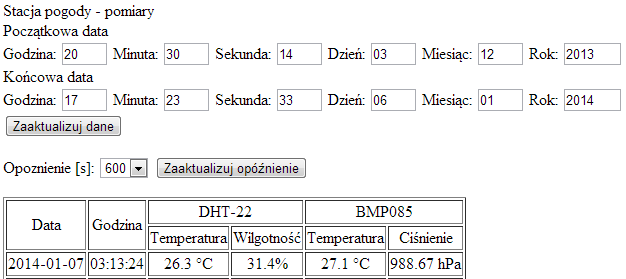
\includegraphics[scale=0.95]{strona}
\caption{Stworzona strona internetowa}
\label{fig:strona}
\end{figure}

Wykresy do pomiarów zostały wykonany przy pomocy biblioteki wykonanej w technologii JavaScript o nazwie Flot.